\documentclass{beamer}
\usetheme{Warsaw}
\usepackage[T1]{fontenc}
\usepackage{alltt}
\usepackage{listings}
\usepackage{graphicx}
\usepackage{perpage}[footmisc] %the perpage package
\MakePerPage{footnote}
\AtBeginSection[]{
  \begin{frame}
  \vfill
  \centering
  \begin{beamercolorbox}[sep=8pt,center,shadow=true,rounded=true]{title}
    \usebeamerfont{title}\insertsectionhead\par%
  \end{beamercolorbox}
  \vfill
  \end{frame}
}
\setbeamertemplate{navigation symbols}{}
\addtobeamertemplate{navigation symbols}{}{%
    \usebeamerfont{footline}%
    \usebeamercolor[fg]{footline}%
    \hspace{1em}%
    \insertframenumber/\inserttotalframenumber
}
\setbeamertemplate{headline}{}
\makeatletter
\def\verbatim@font{\footnotesize\ttfamily}
\makeatother
\newcommand{\credit}[1]{\par\hfill \tiny Credit:~\itshape#1}


\title[XDP]{XDP}
\author{Linos Giannopoulos}
\date{March 28, 2019}
\begin{document}

\begin{frame}
\titlepage
\end{frame}

\begin{frame}[c]
  \begin{figure}
    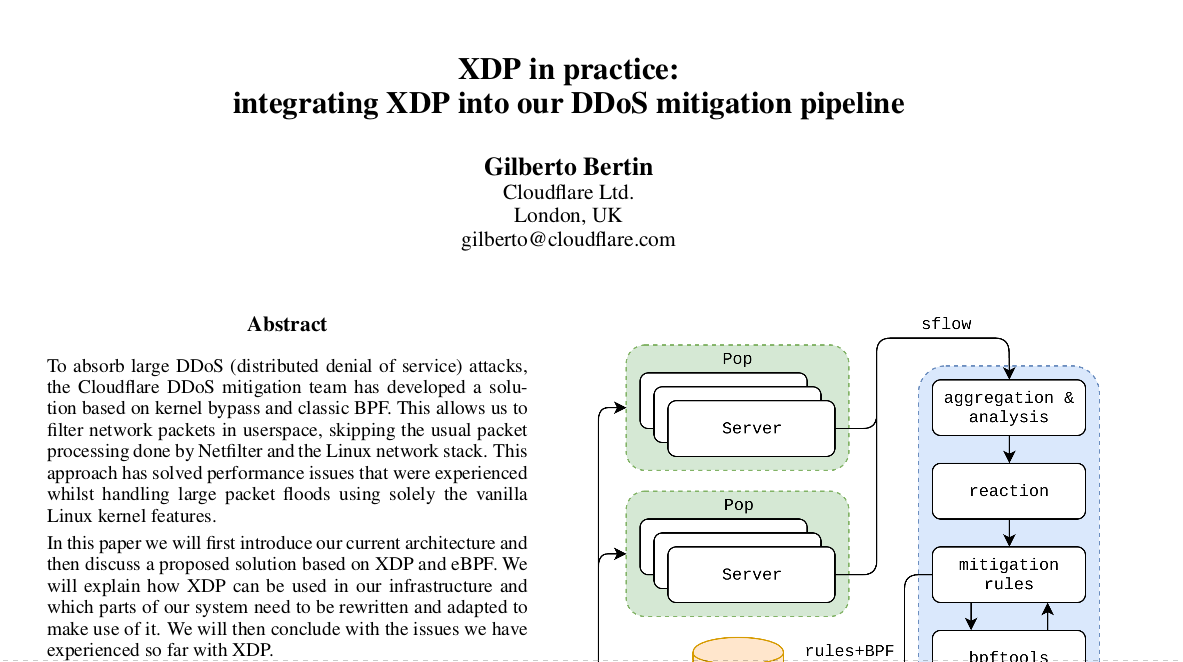
\includegraphics[width=\textwidth]{./paper.png}
  \end{figure}
\end{frame}

\begin{frame}{Agenda}
  \begin{itemize}
    \item cBPF
    \item eBPF
    \item XDP
    \item DDoS Mitigation Pipeline
  \end{itemize}
\end{frame}

\section{cBPF}
\begin{frame}{cBPF}
Berkeley Packet Filter
\begin{itemize}
\item \textit{The BSD Packet Filter: A New Architecture for User-level Packet Capture}
\item Avoid needless copying of packets
\item Register-based VM in-kernel
\item Filter packets as early as possible
\end{itemize}
\end{frame}

\begin{frame}{cBPF}
  \begin{figure}
    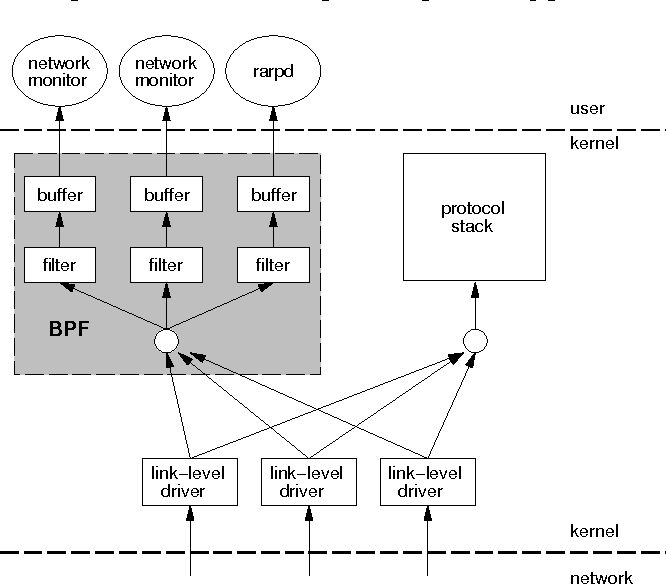
\includegraphics[width=0.85\textwidth]{./cbpf.png}
  \end{figure}
\end{frame}

% \begin{frame}[fragile]
%   \frametitle{cBPF}
%   \begin{verbatim}
% # lgian[~] tcpdump -i any tcp -d
% (000) ldh      [14]
% (001) jeq      #0x86dd          jt 2 jf 7
% (002) ldb      [22]
% (003) jeq      #0x6             jt 10 jf 4
% (004) jeq      #0x2c            jt 5 jf 11
% (005) ldb      [56]
% (006) jeq      #0x6             jt 10 jf 11
% (007) jeq      #0x800           jt 8  jf 11
% (008) ldb      [25]
% (009) jeq      #0x6             jt 10 jf 11
% (010) ret      #262144
% (011) ret      #0

% # lgian[~] strace -e trace=setsockopt tcpdump -i any tcp
% ...
%   setsockopt(3, SOL_SOCKET, SO_ATTACH_FILTER, 
%     {len=12, filter=0x5630ba569dd0}, 16) = 0
%   \end{verbatim}
% \end{frame}

\section{eBPF}
\begin{frame}{eBPF}
  What changed
  \begin{itemize}
    \item Extended ISA for modern CPUs
    \item More registers (from 2 to 10)
    \item JIT compiler bytecode to native code
  \end{itemize}

  New concepts
  \begin{itemize}
    \item eBPF Maps shared between user and kernel space
    \item eBPF Verifier
  \end{itemize}
\end{frame}

\begin{frame}{eBPF Map Types}
  \begin{columns}
    \begin{column}{0.5\textwidth}
      \begin{itemize}
        \item Hash
        \item Array
        \item Tail Call Array
        \item Per-CPU Hash/Array
        \item Stack Trace
      \end{itemize}
    \end{column}
    \begin{column}{0.5\textwidth}
        \begin{center}
          \begin{itemize}
            \item LRU (per-CPU) Hash
            \item Longest-Prefix Matching Trie
            \item Array/Hash of Maps
            \item Net device Map
            \item Socket Map
            \item ...
          \end{itemize}
        \end{center}
    \end{column}
  \end{columns}
\end{frame}

\begin{frame}{eBPF Verifier}
  We essentially run userspace programs in the kernel. 
  \break

  How can we ensure an eBPF program won't cause a kernel panic or read/write arbitrary kernel memory?
  \break

  \pause

  Restrictions:

  \begin{itemize}
  \item 4096 instructions per program
  \item No loops
  \item No unreachable instructions
  \item Cannot read uninitialized registers
  \item Cannot read any arbitrary memory
  \item No out-of-bounds jumps
  \item Everything needs to be inlined (no function calls or shared library calls)
  \item Only calls to BPF Helpers ( BPF to BPF is also allowed on newer kernel versions )
  \end{itemize}
\end{frame}

\begin{frame}[fragile]
  \frametitle{(some) eBPF Helper Functions}
  \textit{uapi/linux/bpf.h~}
  \begin{verbatim}
  #define __BPF_FUNC_MAPPER(FN)   \
    FN(map_lookup_elem),    \
    FN(map_update_elem),    \
    FN(map_delete_elem),    \
    ...
    FN(ktime_get_ns),   \
    FN(trace_printk),   \
    FN(get_prandom_u32),    \
    FN(skb_store_bytes),    \
    FN(l3_csum_replace),    \
    FN(tail_call),      \
    FN(xdp_adjust_head),    \
    FN(xdp_adjust_meta),    \
    ...
\end{verbatim}
\end{frame}

\begin{frame}{eBPF}
  Some use cases:
  \begin{itemize}
    \item Tracing (kprobes/uprobes/tracepoints)\footnotemark
    \item Networking (tc/XDP)
    \item Security (seccomp/IDS/DDoS)
  \end{itemize}
  \footnotetext[1]{\url{https://www.youtube.com/watch?v=w8nFRoFJ6EQ}}
\end{frame}

\section{XDP}
\begin{frame}{Receiving a packet}
  \begin{figure}
    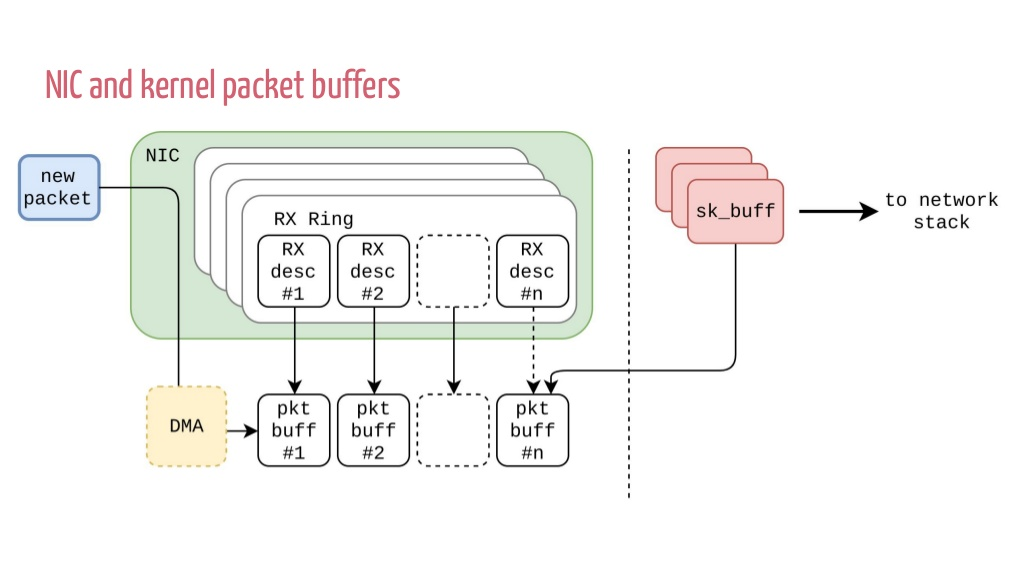
\includegraphics[width=0.85\textwidth]{./dma-nic.jpg}

  \end{figure}
\end{frame}
\begin{frame}{XDP}
  eXpress Data Path
  \begin{itemize}
    \item High-performance packet processing
    \item Runs eBPF programs at the earliest possible point (before sk\_buffer allocations)
    \item In concert with the kernel (no userspace bypass or out-of-tree kernel modifications)
    \item Driver dependant
    \item Verdicts: XDP\_DROP, XDP\_PASS, XDP\_TX, XDP\_ABORTED, XDP\_REDIRECT
  \end{itemize}
\end{frame}

\begin{frame}{XDP}
  Use cases:
  \begin{itemize}
    \item Firewalling (Cillium\footnotemark[1])
    \item DDoS
    \item Load balancing (Katran\footnotemark[2])
    \item Monitoring
  \end{itemize}
  \footnotetext[1]{\tiny\url{https://cilium.io/}}
  \footnotetext[2]{\tiny\url{https://code.fb.com/open-source/open-sourcing-katran-a-scalable-network-load-balancer/}}
\end{frame}

\begin{frame}[fragile]
  \frametitle{XDP Example}
  \begin{verbatim}
    #include <linux/bpf.h>
    #include <linux/if_ether.h>
    #include <linux/ip.h>
    #define SEC(NAME) __attribute__((section(NAME), used))

    SEC("dropper")
    int xdp(struct xdp_md *ctx)
    {
        void *data = (void *)(long)ctx->data;
        void *data_end = (void *)(long)ctx->data_end;
        struct iphdr *ip = data + sizeof(struct ethhdr);

        // +1 is sizeof(struct iphdr)
        if (ip + 1 > data_end)
            return XDP_ABORTED;

        if(ip->saddr == 59017107){ // Binary format of "147.135.132.3"
            return XDP_DROP;
        }
        return XDP_PASS;
    }
  \end{verbatim}
\end{frame}

\begin{frame}{XDP Load Program}
  \begin{figure}
    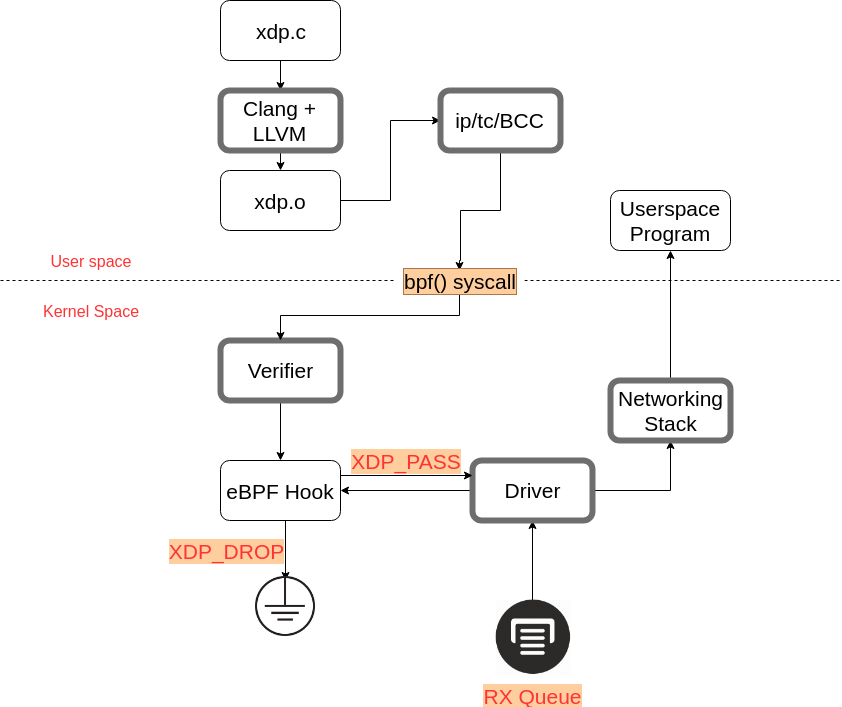
\includegraphics[width=0.85\textwidth]{./xdp_workflow.png}

  \end{figure}
\end{frame}

% \begin{frame}{XDP Load Program}
%   \begin{itemize}
%     \item Write C Program
%     \item clang -O2 -target bpf -c xdp.c -o xdp.o
%     \item ip link set dev eth0 (xdpgeneric|xdpdrv|xdpoffload) obj xdp.o sec <section-name>
%   \end{itemize}
% \end{frame}

\begin{frame}{XDP vs Everything}
  \Large{What about IPtables?}
\end{frame}

\begin{frame}{XDP vs Everything}
  Test bench
  \begin{itemize}
    \item 10GbE Intel NIC
    \item Generate 14Mpps tiny UDP packets (pktgen)
    \item Randomized source IP/Port
    \item Traffic is steered towards a single CPU
    \item Measure number of packets handled by the kernel on that CPU
  \end{itemize}

  \ \\
  \pause
  \textbf{\textit{How fast can we drop packets?}}
\end{frame}

\begin{frame}{XDP vs Everything}
  \begin{figure}
    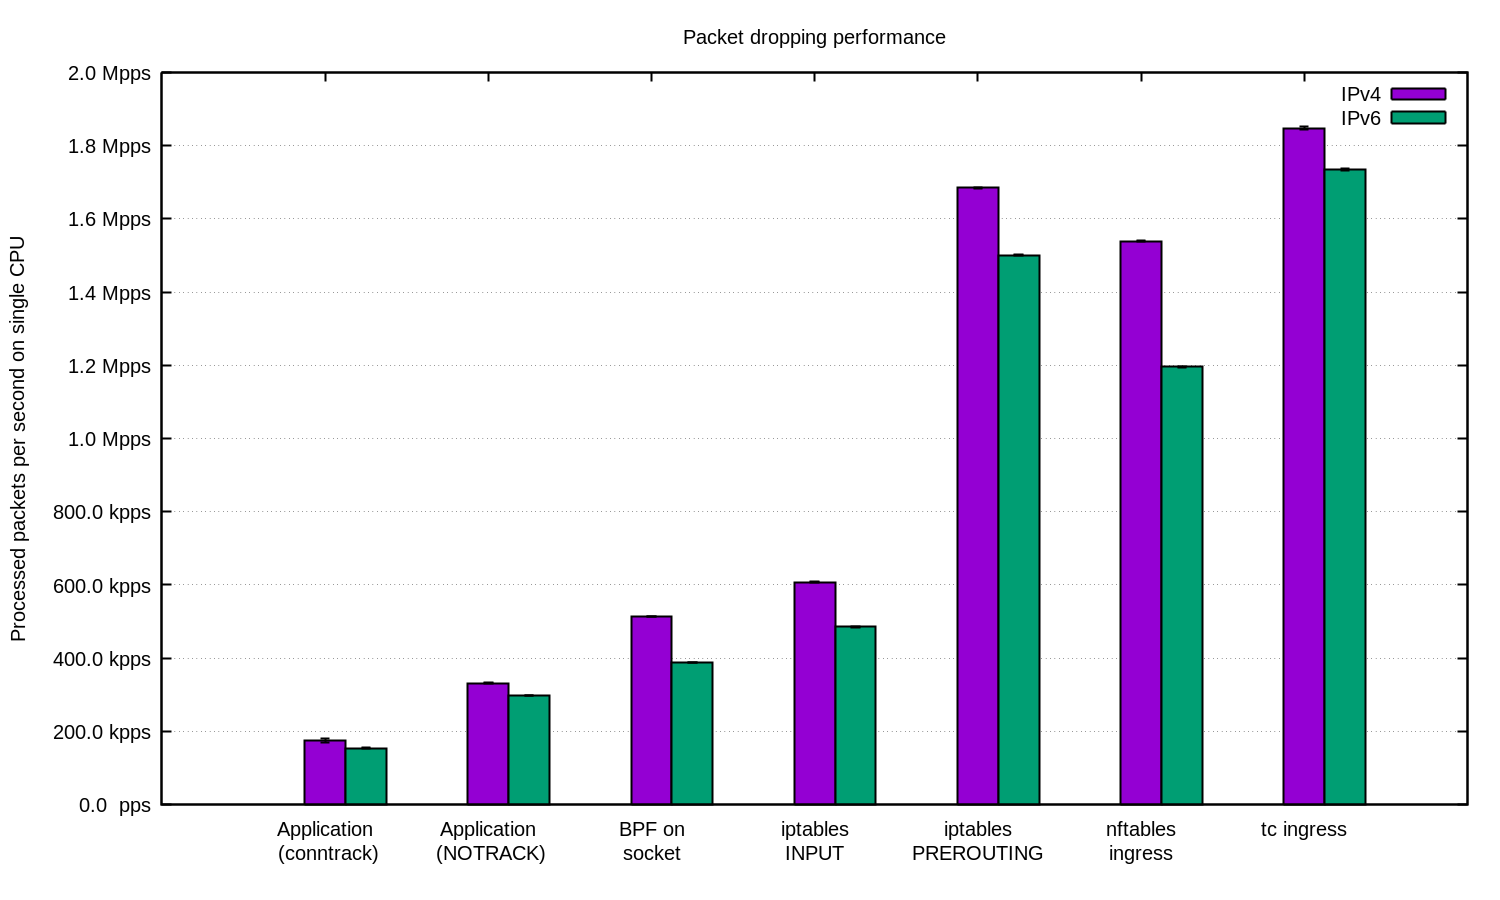
\includegraphics[width=1.1\textwidth]{./no_xdp.png}
  \end{figure}
\end{frame}

\begin{frame}{XDP vs Everything}
  \begin{figure}
    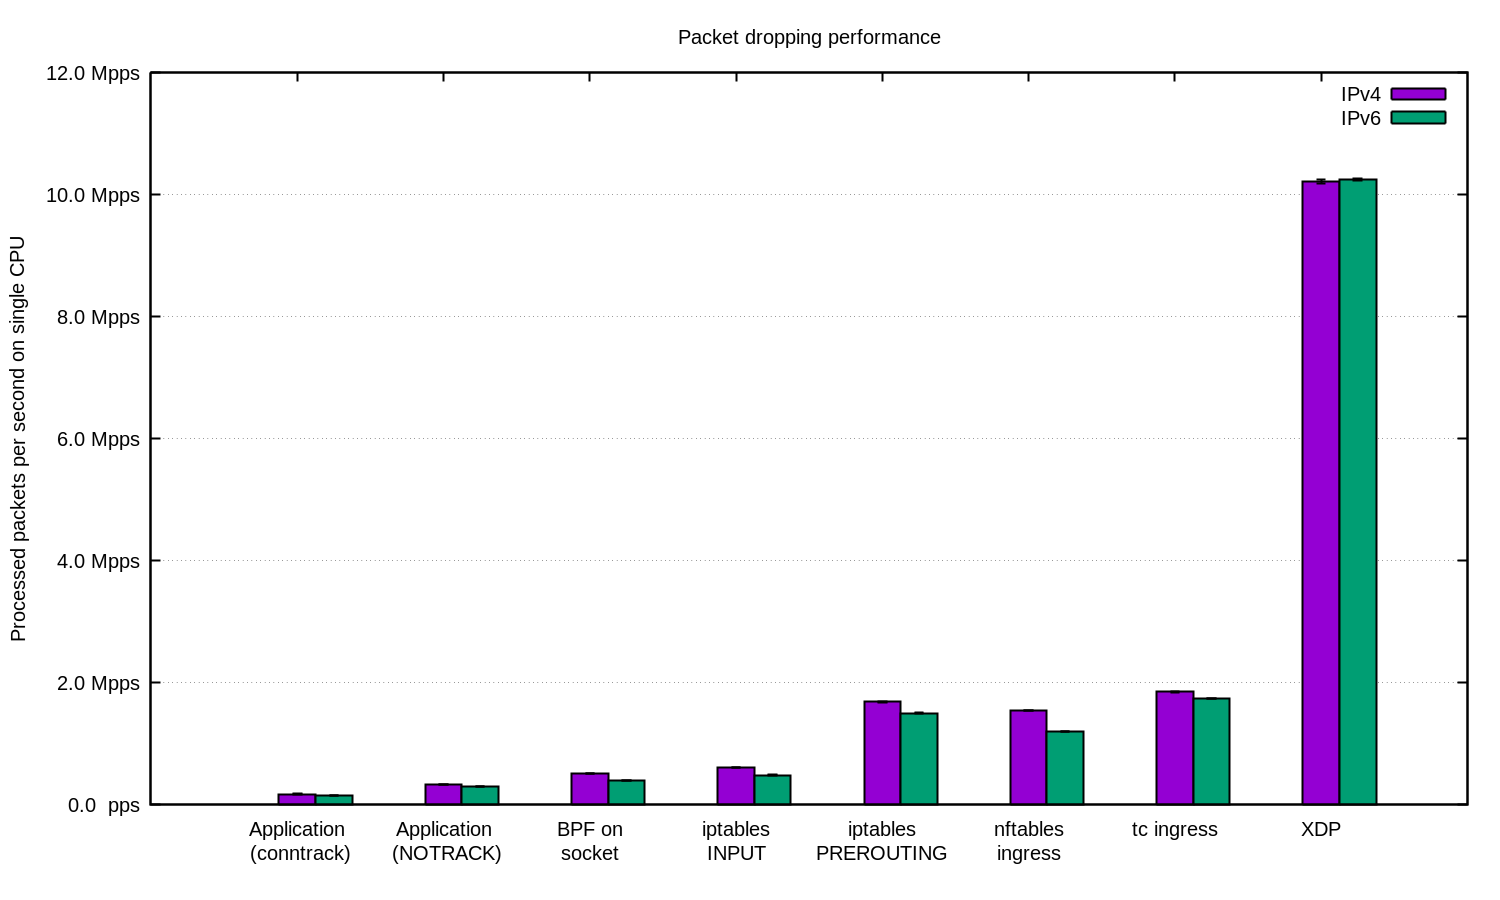
\includegraphics[width=1.1\textwidth]{./with_xdp.png}
  \end{figure}
\end{frame}

\begin{frame}{GRNET's testbed}
  \begin{figure}
    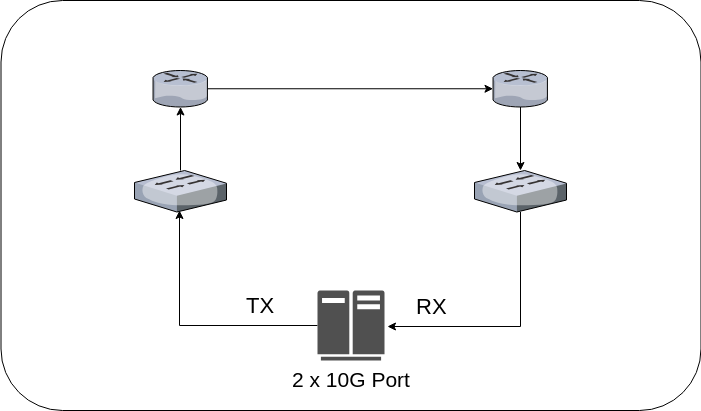
\includegraphics[width=1\textwidth]{./testbench.png}
  \end{figure}
\end{frame}

\begin{frame}{Our results}
  \begin{figure}
    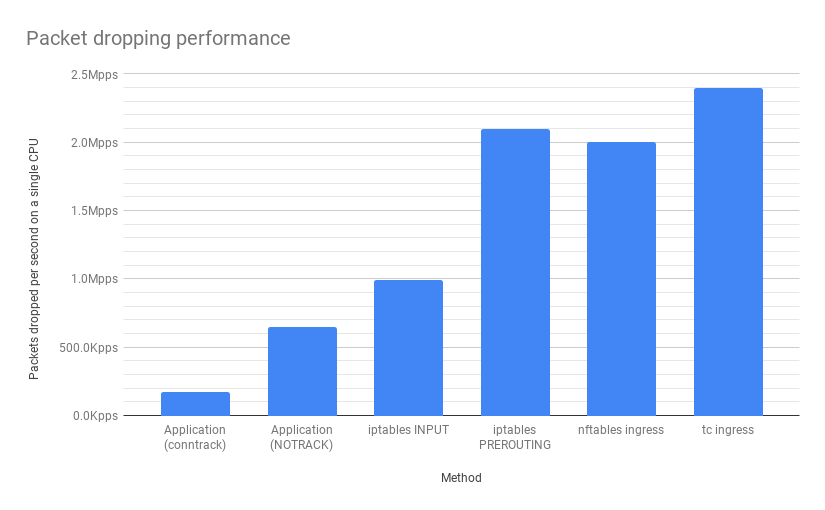
\includegraphics[width=1.1\textwidth]{./custom_no_xdp.png}
  \end{figure}
\end{frame}

\begin{frame}{Our results}

  \begin{figure}
    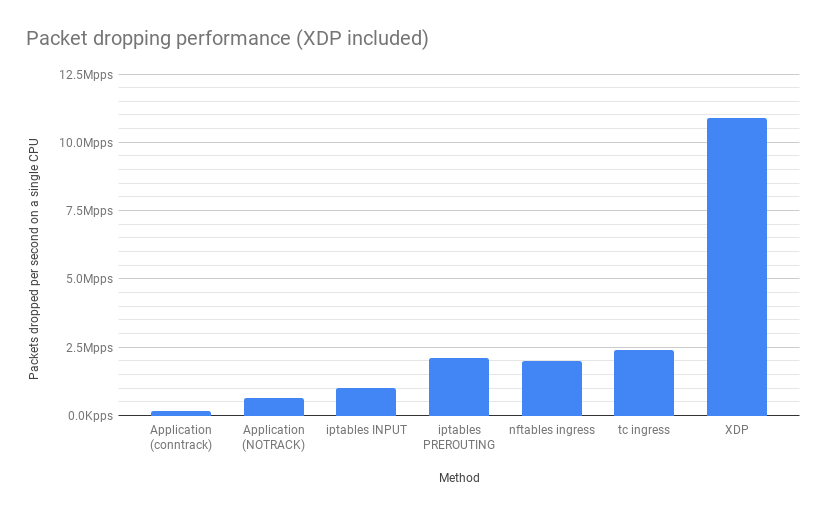
\includegraphics[width=1.1\textwidth]{./custom_xdp.png}
  \end{figure}
\end{frame}

\section{DDoS Pipeline}
\begin{frame}{Overview of Pipeline}
  \begin{itemize}
    \item Traffic sampling
    \item Traffic aggregation and analysis
    \item Attack reaction
  \end{itemize}
\end{frame}

\begin{frame}{Some things to note}
  \begin{itemize}
    \item DDoS Attacks that our uplink can handle
    \item If that's not the case:
      \begin{itemize}
        \item Anycast with different PoPs
        \item Flowspec
      \end{itemize}
    \item Flowspec has its limitations
    \item Software and not hardware limitations
  \end{itemize}
\end{frame}

\begin{frame}{Traffic sampling}
  In contrast with an IDS, sampling instead of working on the whole traffic is crucial here.
  \begin{itemize}
    \item Use \textit{NFLOG (+Statistic)}
    \item Userspace daemon to process packet
  \end{itemize}
  \pause
    \textit{Issue:} no visibility in the dropped traffic
\end{frame}

\begin{frame}{Traffic sampling}
  Sample before drop rules - in XDP
  \begin{itemize}
    \item Copy sampled packet to perf event buffer (xdp\_event\_output)
    \item Userspace daemon to obtain the packet
  \end{itemize}
\end{frame}

\begin{frame}{Traffic aggregation and analysis}
  How do we categorize traffic?
  \pause
  \begin{figure}
    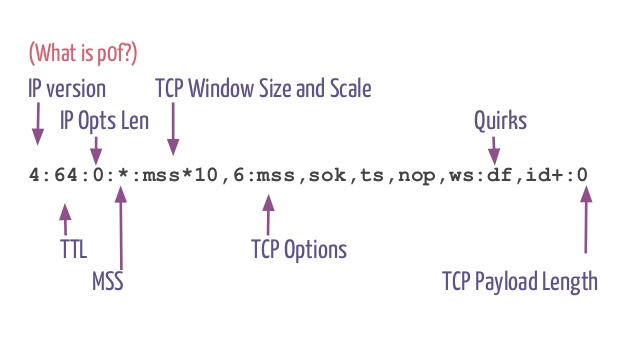
\includegraphics[width=\linewidth]{./p0f.jpg}
    \credit{https://www.slideshare.net/InfoQ/xdp-in-practice-ddos-mitigation-cloudflare}
  \end{figure}
\end{frame}

\begin{frame}{Traffic aggregation and analysis}
  Traffic aggregated into groups
  \begin{itemize}
    \item TCP SYNs, TCP ACKs, UDP/DNS
    \item Destination IP/Port
    \item Known attack vectors and other heuristics
  \end{itemize}
\end{frame}

\begin{frame}[fragile]
\frametitle{p0f -> XDP}
\begin{verbatim}
$ ./p0f2ebpf.py --ip 1.2.3.4 --port 1234 
    '4:64:0:*:mss*10,6:mss,sok,ts,nop,ws:df,id+:0'

static inline int match_p0f(void *data, void *data_end) {
    struct ethhdr *eth_hdr;
    struct iphdr *ip_hdr;
    struct tcphdr *tcp_hdr;
    u8 *tcp_opts;

    eth_hdr = (struct ethhdr *)data;
    if (eth_hdr + 1 > (struct ethhdr *)data_end)
        return XDP_ABORTED;
    if_not (eth_hdr->h_proto == htons(ETH_P_IP))
        return XDP_PASS;


\end{verbatim}
\end{frame}

\begin{frame}[fragile]
\frametitle{p0f -> XDP}
\begin{verbatim}
    ip_hdr = (struct iphdr *)(eth_hdr + 1);
    if (ip_hdr + 1 > (struct iphdr *)data_end)
        return XDP_ABORTED;
    if_not (ip_hdr->daddr == htonl(0x1020304))
        return XDP_PASS;
    if_not (ip_hdr->version == 4)
        return XDP_PASS;
    if_not (ip_hdr->ttl <= 64)
        return XDP_PASS;
    if_not (ip_hdr->ttl > 29)
        return XDP_PASS;
    if_not (ip_hdr->ihl == 5)
        return XDP_PASS;
    if_not ((ip_hdr->frag_off & IP_DF) != 0)
        return XDP_PASS;
    if_not ((ip_hdr->frag_off & IP_MBZ) == 0)
        return XDP_PASS;
\end{verbatim}
\end{frame}

\begin{frame}[fragile]
  \frametitle{p0f -> XDP}
  \begin{verbatim}
    tcp_hdr = (struct tcphdr*)((u8 *)ip_hdr +
    ip_hdr->ihl * 4);
    if (tcp_hdr + 1 > (struct tcphdr *)data_end)
        return XDP_ABORTED;
    if_not (tcp_hdr->dest == htons(1234))
        return XDP_PASS;
    if_not (tcp_hdr->doff == 10)
        return XDP_PASS;
    if_not ((htons(ip_hdr->tot_len) - (ip_hdr->ihl * 4) - (tcp_hdr->doff * 4)) == 0)
        return XDP_PASS;

    ...

    return XDP_DROP;
}
  \end{verbatim}
\end{frame}

\begin{frame}{Pipeline}
  \begin{figure}
    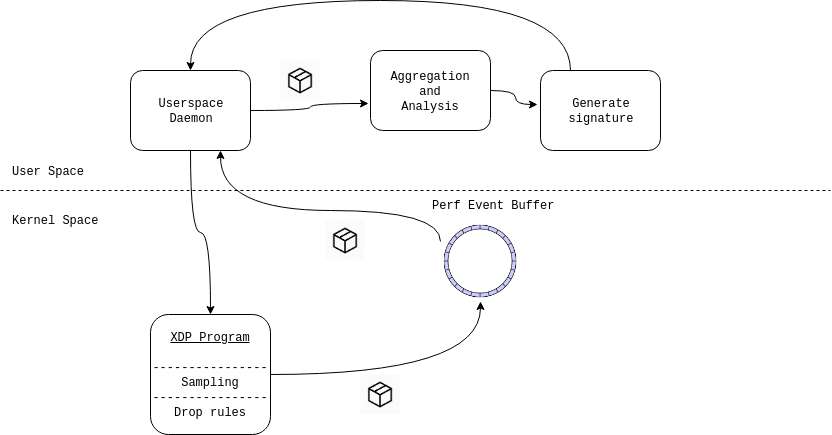
\includegraphics[width=\linewidth]{./ddos.png}
  \end{figure}
\end{frame}

\begin{frame}{A more realistic test}
  \begin{itemize}
    \item Generate ~8.7Mpps\footnotemark TCP SYN packets (trafgen)
    \item Randomized source IP/Port
    \item Traffic is steered towards a single CPU
    \item Measure number of packets handled by the kernel on that CPU
  \end{itemize}
  \footnotetext[1]{We can do better!}
\end{frame}

\begin{frame}{A more realistic test}
  Methodology:
  \begin{itemize}
    \item Sample traffic
    \item Feed samples to p0f
    \item Grab signature
    \item Generate XDP program to drop the malicious traffic
    \item Attach it to XDP hook
  \end{itemize}
\end{frame}

\begin{frame}[plain]
        \makebox[\linewidth]{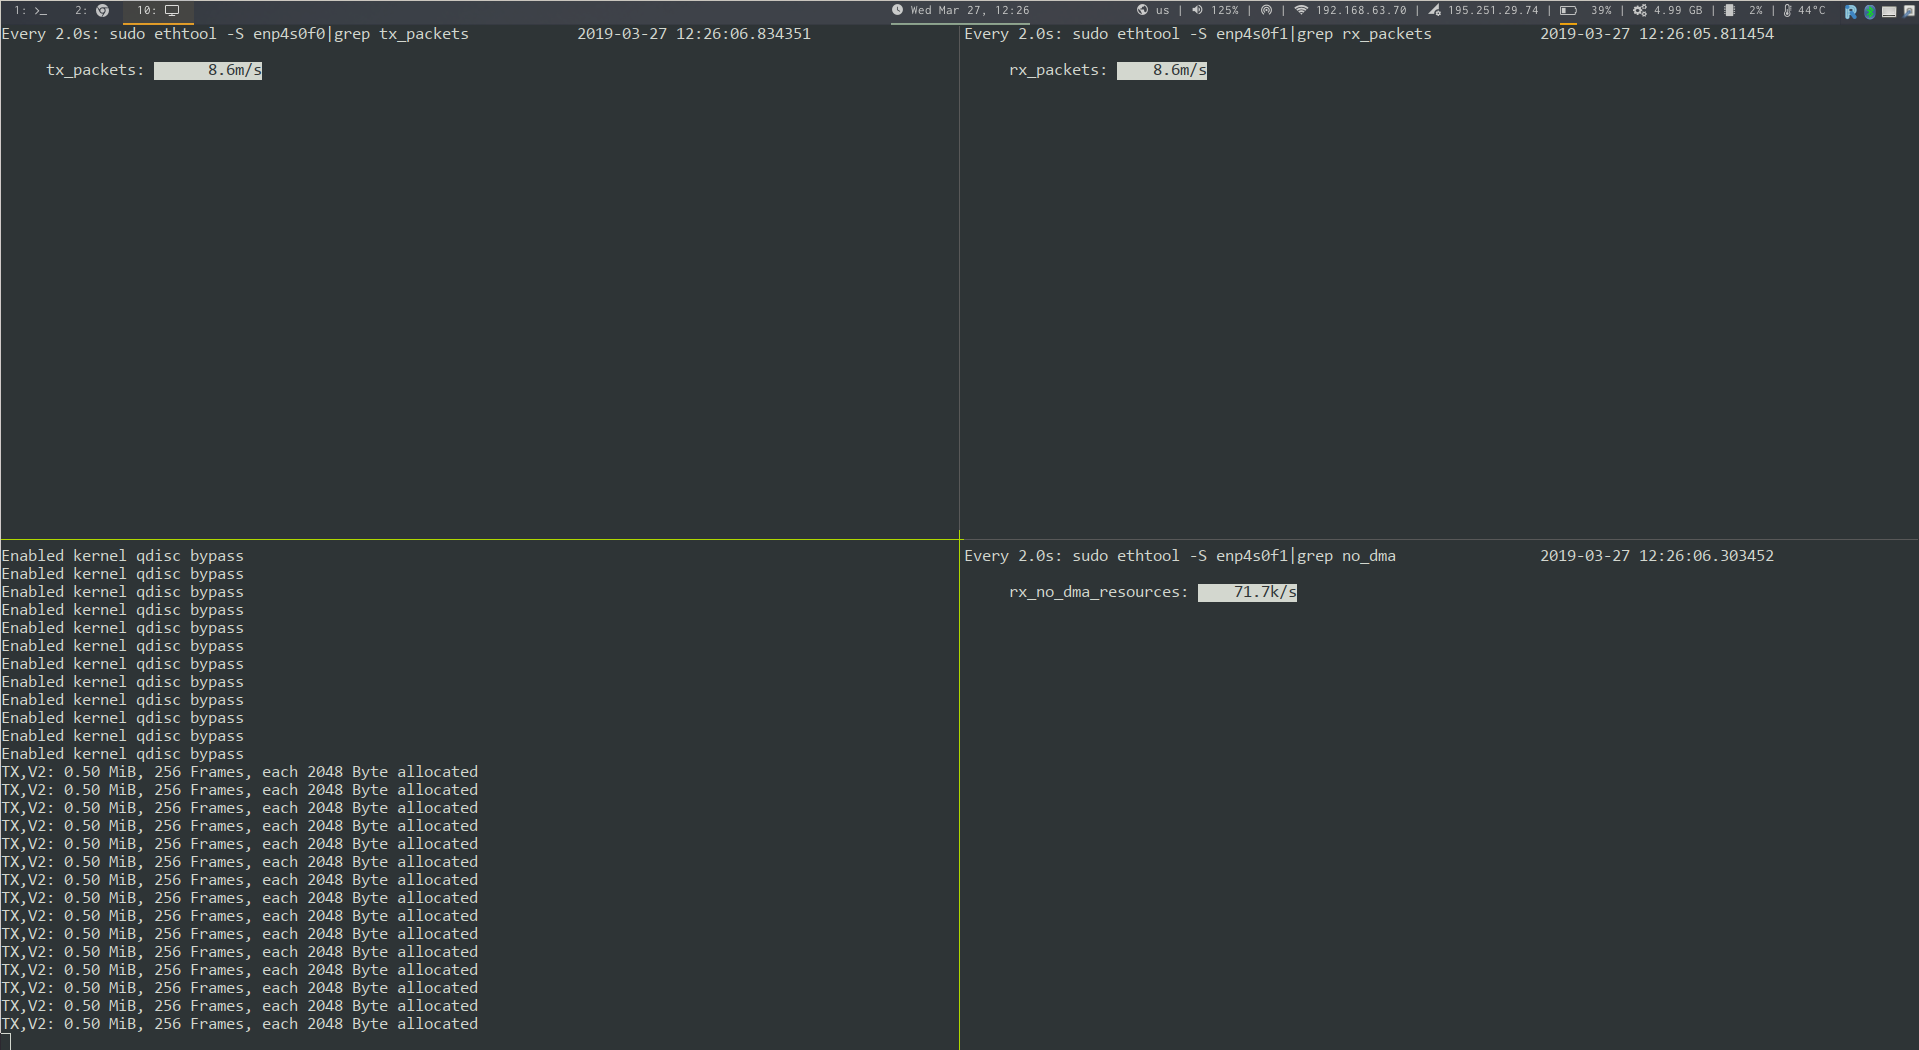
\includegraphics[width=\paperwidth]{./trafgen.png}}
\end{frame}

\begin{frame}{}
  \begin{center}
    \Huge Questions?
  \end{center}

\end{frame}
\end{document}
